\documentclass[12pt]{report}
\setlength{\textwidth}{6.5 in}
\setlength{\evensidemargin}{0 in}
\setlength{\oddsidemargin}{0 in}
\setlength{\textheight}{9.4 in }
\setlength{\topmargin}{-0.7 in}
\pagestyle{myheadings}
\markboth{\em EE264: Homework \#03}{\em EE264: Homework \#03}
\usepackage[pdftex]{graphicx} \usepackage{eso-pic}
\usepackage{amsmath}
\usepackage{amssymb}
\usepackage{graphicx}
\usepackage{ifthen}
\usepackage{tikz}
\usepackage{pgfplots}
\usepackage{array}  % for table column M
\usepackage{makecell} % to break line within a cell
\usepackage{verbatim}
\usepackage{epstopdf}
\usepackage{amsfonts}
\usepackage{xcolor}
\usepackage{subcaption}
\usepackage{pdfpages}
\usepackage{setspace}
\usepackage{placeins} % for FloatBarrier
\usepackage[makeroom]{cancel}
\usepackage[absolute,overlay]{textpos}
%\captionsetup{compatibility=false}
%\usepackage{dsfont}
\usepackage[absolute,overlay]{textpos}
\usetikzlibrary{calc}
\usetikzlibrary{pgfplots.fillbetween, backgrounds}
\usetikzlibrary{positioning}
\usetikzlibrary{arrows}
\usetikzlibrary{pgfplots.groupplots}
\usetikzlibrary{arrows.meta}
\usetikzlibrary{plotmarks}
\usetikzlibrary{calc, angles,quotes}
\usetikzlibrary{decorations.markings}

\usepgfplotslibrary{groupplots}
\pgfplotsset{compat=newest} 

\DeclareGraphicsExtensions{.pdf,.eps,.png}

\DeclareMathOperator{\E}{\mathbb{E}} % expectation

\definecolor{blue2}{RGB}{51, 105, 232}  
\definecolor{red2}{RGB}{213, 15, 37}  
\definecolor{green2}{RGB}{0, 153, 37}  


%%%%%%%%%%%%% SOLUTIONS %%%%%%%%%%%%%%%%%
\def\SOLUTIONS{0} % change to 1 to produce solutions
\def\SolutionsColor{red2}
%%%%%%%%%%%%%%%%%%%%%%%%%%%%%%%%%%%%%%%%%



\begin{document}
\thispagestyle{empty}
\begin{centering}
	{\large Stanford University}\\
	{\large EE 264: Digital Signal Processing}\\
	{\large Summer, 2018} \\
	\mbox{}\\
	{\large Homework \#03}\\
	\mbox{}\\
\end{centering}
\noindent Date assigned:  July 13, 2018 \hfill
Date due: July 20, 2018\\
\noindent \rule{6.5 in}{0.5pt}
%\mbox{}\\
\noindent {\bf Reading:}  Problems 2-5 need lecture notes 4, which will be finished in class on Monday, July 16, 2018. \\
\noindent {\bf Homework submission:}  Please submit your solutions on Gradescope. Create a single .pdf file containing all your analytical derivations, sketches, plots, and Matlab code (if any). \\
\noindent
\rule{6.5 in}{0.5pt}
\mbox{}\\



\noindent {\bf Problem 1: Poles and zeros of the deterministic autocorrelation function (30 points)}

As discussed in class, the deterministic autocorrelation function of an LTI system with impulse response $h[n]$ is defined by
\begin{equation}
c_{hh}[n] = h[n] \ast h^*[-n].
\end{equation}

For this problem, consider that $h[n]$ is \underline{causal} and that the pole-zero diagram of its $z$-transform, $H(z)$, is shown in Figure~\ref{fig:pole-zero}a.

\begin{description}
\item{(a)} (8 points)
Sketch the pole-zero diagram of the $z$-transform of the deterministic autocorrelation function $C_{hh}(z) \Longleftrightarrow c_{hh}[n]$. Use the empty diagram of Figure~\ref{fig:pole-zero}b for your sketch. 

\textit{Hint:} First write $C_{hh}(z)$ in terms of $H(z)$ using the properties of the $z$-transform.

\begin{figure}[!h]
\centering
	\resizebox{\textwidth}{!}{\begin{tikzpicture}
\begin{axis}[
name=plot1,
axis equal,
axis lines*=middle,
enlargelimits = false, clip=true,
xmin=-1.39,
xmax=1.39,
ymin=-1.10,
ymax=1.10,
axis line style={->,>=stealth},
xlabel={$\mathrm{Re}\{z\}$},
ylabel={$\mathrm{Im}\{z\}$},
every axis x label/.style={
at={(ticklabel* cs:1)},
anchor=north,
},
every axis y label/.style={
at={(ticklabel* cs:1)},
anchor=south,
},
xtick=1, ytick=\empty,
xticklabel style={xshift=0.1cm},
every outer y axis line/.append style={white!15!black},
every y tick label/.append style={font=\color{white!15!black}},
legend style={draw=white!15!black,fill=white,legend cell align=left}]
\draw (axis cs:0,0) circle [black!50, dashed, line width=2pt, radius=1];
\if\SOLUTIONS1
	\addplot [line width=1pt,mark=x, only marks, mark size = 3pt]
	table[row sep=crcr]{
		0.56569 0.56569 \\
		0.56569 -0.56569 \\
	};
	
	\addplot [line width=1pt,mark=*, only marks, mark size = 3pt, mark options={fill=white}]
	table[row sep=crcr]{
		-0.88388 0.88388 \\
		-0.88388 -0.88388 \\
	};
\fi
\end{axis}

\begin{axis}[
name=plot2,
at= (plot1.east), anchor=west, xshift=1cm,
%at=(plot1.below south east), anchor=above north east,
axis equal,
axis lines*=middle,
enlargelimits = false, clip=true,
xmin=-1.39,
xmax=1.39,
ymin=-1.10,
ymax=1.10,
axis line style={->,>=stealth},
xlabel={$\mathrm{Re}\{z\}$},
ylabel={$\mathrm{Im}\{z\}$},
every axis x label/.style={
	at={(ticklabel* cs:1)},
	anchor=north,
},
every axis y label/.style={
	at={(ticklabel* cs:1)},
	anchor=south,
},
xtick=1, ytick=\empty,
xticklabel style={xshift=0.1cm},
every outer y axis line/.append style={white!15!black},
every y tick label/.append style={font=\color{white!15!black}},
legend style={draw=white!15!black,fill=white,legend cell align=left}]
\draw (axis cs:0,0) circle [black!50, dashed, line width=2pt, radius=1];
\if\SOLUTIONS1
  \addplot [\SolutionsColor, line width=1pt,mark=x, only marks, mark size = 3pt]
  table[row sep=crcr]{
      0.56569 0.56569 \\
      0.56569 -0.56569 \\
      0.8839 +0.8839 \\
      0.8839 -0.8839 \\
  };

  \addplot [\SolutionsColor, line width=1pt,mark=*, only marks, mark size = 3pt, mark options={fill=white}]
  table[row sep=crcr]{
      -0.88388 0.88388 \\
      -0.88388 -0.88388 \\
      -0.5657 +0.5657 \\
      -0.5657 -0.5657  \\
  };
\fi
\end{axis}

\node[below] at (plot1.south) {(a)};
\node[below] at (plot2.south) {(b)};
\end{tikzpicture}}
    \caption{Pole-zero diagram of (a) $H(z)$ and (b) $C_{hh}(z)$.} \label{fig:pole-zero}
\end{figure}


\if\SOLUTIONS1
{\color{\SolutionsColor}
Using the conjugate and time reversal properties of the $z$-transform, we can write: $h^*[-n] \Longleftrightarrow H^*(1/z^*)$. Consequently,
\begin{equation*}
C_{hh}(z) = H(z)H^*(1/z^*)
\end{equation*}

From this equation we see that all the poles and zeros of $H(z)$ are also poles and zeros of $C_{hh}(z)$. 

Moreover, suppose that $p$ is a pole of $H(z)$. Then, $H(z)$ must have a factor $\frac{1}{z-p}$:
\begin{equation}
\frac{1}{z-p} \implies \frac{1}{(1/z^*-p)^*}  = \frac{z}{p^*(1/p^*-z)} 
\end{equation}
Therefore, for each pole $p$ of $H(z)$, $C_{hh}(z)$ has a pole at $p$,  another pole at $1/p^*$, and a new zero at $z = 0$. We can use the same arguments to show that for every zero $c$ of $H(z)$, $C_{hh}(z)$ has a zero at $c$, another zero at $1/c^*$, and a new pole at $z = 0$. Now we're ready to draw the zero-pole plot
}
\else\vspace{7cm}
\fi

\item{(b)} (4 points) In part (a) you may have noticed that $C_{hh}(z)$ has poles outside the unit circle. Does that mean that $C_{hh}(z)$ is unstable? Justify your answer. 

\textit{Hint:} $h[n]$ is causal, but is $c_{hh}[n]$ causal?

\if\SOLUTIONS1
{\color{\SolutionsColor}
$c_{hh}[n]$ is not causal, since it is the convolution of a causal ($h[n]$) and an anti-causal ($h^*[-n]$) sequence. Therefore, the ROC of  $C_{hh}(z)$ is the annulus (ring-shaped region) between two circles defines by the poles.  This region includes the unit circle, and therefore $C_{hh}(z)$ is stable.
}
\else\vspace{3cm}
\fi




\item{(c)} (7 points) Suppose that a \underline{white} noise signal $x[n]$ with average power $\sigma_x^2 = 1$ is input to the system $h[n]$. Sketch the PSD of the output noise $y[n] = x[n]\ast h[n]$. Since the pole-zero diagram does not provide information about the gain, the first and last points of the magnitude response are already included. Note that the magnitude in this plot is in log scale.

\textit{Note:} your sketch does not need to be perfect to receive full credit, but be sure to indicate the most relevant points.

\begin{figure}[!h]
	\centering
	\resizebox{0.6\textwidth}{!}{\begin{tikzpicture}
\begin{axis}[
axis lines*=middle,
enlargelimits = upper, clip=true,
scale only axis,
axis line style={->,>=stealth},
xlabel={$\omega$},
ylabel={$10\log_{10}(\Phi_{yy}(e^{j\omega}))$},
every axis x label/.style={
	at={(ticklabel* cs:1)},
	xshift=-0.2cm,
	anchor=north,
},
every axis y label/.style={
	at={(ticklabel* cs:1)},
	xshift=0.4cm,
	%yshift=0.35cm,
	anchor=south,
},
every outer x axis line/.append style={white!15!black},
every x tick label/.append style={font=\color{white!15!black}},
xmin=0, xmax=1,
ymin=-35, ymax=10,
xtick={0, 0.25, 0.5, 0.75, 1},
xticklabels ={$0$, $\pi/4$, $\pi/2$, $3\pi/4$, $\pi$},
ytick={-30,-20,...,10},
xmajorgrids,
ymajorgrids,
every outer y axis line/.append style={white!15!black},
every y tick label/.append style={font=\color{white!15!black}},
legend style={draw=white!15!black,fill=white,legend cell align=left}]
\addplot [color=black, only marks, mark=*, mark size=3pt, line width=1.5pt, forget plot]
table[row sep=crcr]{
	0 -1.9287e-15 \\
    0.99805 -29.4521 \\
};

\if\SOLUTIONS1
\addplot [color=\SolutionsColor, solid, line width=1.5pt, forget plot]
table[row sep=crcr]{
	0 -1.9287e-15 \\
	0.0019531 0.00035131 \\
	0.0039063 0.0014053 \\
	0.0058594 0.0031622 \\
	0.0078125 0.0056224 \\
	0.0097656 0.0087863 \\
	0.011719 0.012655 \\
	0.013672 0.017228 \\
	0.015625 0.022508 \\
	0.017578 0.028495 \\
	0.019531 0.03519 \\
	0.021484 0.042595 \\
	0.023438 0.050712 \\
	0.025391 0.059541 \\
	0.027344 0.069085 \\
	0.029297 0.079346 \\
	0.03125 0.090325 \\
	0.033203 0.10203 \\
	0.035156 0.11445 \\
	0.037109 0.1276 \\
	0.039062 0.14148 \\
	0.041016 0.15609 \\
	0.042969 0.17143 \\
	0.044922 0.18751 \\
	0.046875 0.20433 \\
	0.048828 0.22189 \\
	0.050781 0.2402 \\
	0.052734 0.25926 \\
	0.054688 0.27908 \\
	0.056641 0.29965 \\
	0.058594 0.32098 \\
	0.060547 0.34308 \\
	0.0625 0.36595 \\
	0.064453 0.38959 \\
	0.066406 0.41401 \\
	0.068359 0.43922 \\
	0.070312 0.46521 \\
	0.072266 0.49199 \\
	0.074219 0.51957 \\
	0.076172 0.54795 \\
	0.078125 0.57713 \\
	0.080078 0.60713 \\
	0.082031 0.63794 \\
	0.083984 0.66957 \\
	0.085938 0.70202 \\
	0.087891 0.73531 \\
	0.089844 0.76943 \\
	0.091797 0.80439 \\
	0.09375 0.84019 \\
	0.095703 0.87684 \\
	0.097656 0.91435 \\
	0.099609 0.95271 \\
	0.10156 0.99194 \\
	0.10352 1.032 \\
	0.10547 1.073 \\
	0.10742 1.1148 \\
	0.10938 1.1575 \\
	0.11133 1.2011 \\
	0.11328 1.2456 \\
	0.11523 1.291 \\
	0.11719 1.3372 \\
	0.11914 1.3844 \\
	0.12109 1.4324 \\
	0.12305 1.4813 \\
	0.125 1.5312 \\
	0.12695 1.5819 \\
	0.12891 1.6335 \\
	0.13086 1.6859 \\
	0.13281 1.7393 \\
	0.13477 1.7935 \\
	0.13672 1.8486 \\
	0.13867 1.9046 \\
	0.14062 1.9614 \\
	0.14258 2.0191 \\
	0.14453 2.0776 \\
	0.14648 2.1369 \\
	0.14844 2.1971 \\
	0.15039 2.258 \\
	0.15234 2.3196 \\
	0.1543 2.382 \\
	0.15625 2.4451 \\
	0.1582 2.5089 \\
	0.16016 2.5734 \\
	0.16211 2.6385 \\
	0.16406 2.7041 \\
	0.16602 2.7703 \\
	0.16797 2.8369 \\
	0.16992 2.904 \\
	0.17188 2.9714 \\
	0.17383 3.0392 \\
	0.17578 3.1071 \\
	0.17773 3.1752 \\
	0.17969 3.2434 \\
	0.18164 3.3116 \\
	0.18359 3.3796 \\
	0.18555 3.4474 \\
	0.1875 3.5149 \\
	0.18945 3.5819 \\
	0.19141 3.6483 \\
	0.19336 3.714 \\
	0.19531 3.7787 \\
	0.19727 3.8424 \\
	0.19922 3.9049 \\
	0.20117 3.966 \\
	0.20312 4.0254 \\
	0.20508 4.0831 \\
	0.20703 4.1387 \\
	0.20898 4.1921 \\
	0.21094 4.2429 \\
	0.21289 4.2911 \\
	0.21484 4.3363 \\
	0.2168 4.3783 \\
	0.21875 4.4168 \\
	0.2207 4.4516 \\
	0.22266 4.4823 \\
	0.22461 4.5088 \\
	0.22656 4.5307 \\
	0.22852 4.5479 \\
	0.23047 4.56 \\
	0.23242 4.5668 \\
	0.23437 4.5682 \\
	0.23633 4.5637 \\
	0.23828 4.5534 \\
	0.24023 4.537 \\
	0.24219 4.5143 \\
	0.24414 4.4853 \\
	0.24609 4.4498 \\
	0.24805 4.4077 \\
	0.25 4.359 \\
	0.25195 4.3037 \\
	0.25391 4.2418 \\
	0.25586 4.1733 \\
	0.25781 4.0983 \\
	0.25977 4.017 \\
	0.26172 3.9293 \\
	0.26367 3.8356 \\
	0.26563 3.7359 \\
	0.26758 3.6305 \\
	0.26953 3.5195 \\
	0.27148 3.4032 \\
	0.27344 3.2818 \\
	0.27539 3.1556 \\
	0.27734 3.0248 \\
	0.2793 2.8897 \\
	0.28125 2.7505 \\
	0.2832 2.6075 \\
	0.28516 2.461 \\
	0.28711 2.3112 \\
	0.28906 2.1584 \\
	0.29102 2.0027 \\
	0.29297 1.8446 \\
	0.29492 1.684 \\
	0.29688 1.5214 \\
	0.29883 1.3569 \\
	0.30078 1.1907 \\
	0.30273 1.023 \\
	0.30469 0.85394 \\
	0.30664 0.68374 \\
	0.30859 0.51253 \\
	0.31055 0.34047 \\
	0.3125 0.1677 \\
	0.31445 -0.0056607 \\
	0.31641 -0.17948 \\
	0.31836 -0.35365 \\
	0.32031 -0.52808 \\
	0.32227 -0.70265 \\
	0.32422 -0.8773 \\
	0.32617 -1.0519 \\
	0.32813 -1.2265 \\
	0.33008 -1.4009 \\
	0.33203 -1.575 \\
	0.33398 -1.749 \\
	0.33594 -1.9225 \\
	0.33789 -2.0958 \\
	0.33984 -2.2686 \\
	0.3418 -2.441 \\
	0.34375 -2.6129 \\
	0.3457 -2.7843 \\
	0.34766 -2.9551 \\
	0.34961 -3.1255 \\
	0.35156 -3.2952 \\
	0.35352 -3.4644 \\
	0.35547 -3.633 \\
	0.35742 -3.8009 \\
	0.35938 -3.9682 \\
	0.36133 -4.1349 \\
	0.36328 -4.301 \\
	0.36523 -4.4665 \\
	0.36719 -4.6312 \\
	0.36914 -4.7954 \\
	0.37109 -4.9589 \\
	0.37305 -5.1217 \\
	0.375 -5.284 \\
	0.37695 -5.4455 \\
	0.37891 -5.6065 \\
	0.38086 -5.7668 \\
	0.38281 -5.9265 \\
	0.38477 -6.0856 \\
	0.38672 -6.244 \\
	0.38867 -6.4019 \\
	0.39063 -6.5592 \\
	0.39258 -6.7158 \\
	0.39453 -6.8719 \\
	0.39648 -7.0274 \\
	0.39844 -7.1824 \\
	0.40039 -7.3368 \\
	0.40234 -7.4906 \\
	0.4043 -7.644 \\
	0.40625 -7.7968 \\
	0.4082 -7.9491 \\
	0.41016 -8.1008 \\
	0.41211 -8.2521 \\
	0.41406 -8.4029 \\
	0.41602 -8.5533 \\
	0.41797 -8.7031 \\
	0.41992 -8.8526 \\
	0.42188 -9.0015 \\
	0.42383 -9.1501 \\
	0.42578 -9.2982 \\
	0.42773 -9.446 \\
	0.42969 -9.5933 \\
	0.43164 -9.7403 \\
	0.43359 -9.8868 \\
	0.43555 -10.033 \\
	0.4375 -10.1789 \\
	0.43945 -10.3244 \\
	0.44141 -10.4696 \\
	0.44336 -10.6145 \\
	0.44531 -10.7591 \\
	0.44727 -10.9033 \\
	0.44922 -11.0473 \\
	0.45117 -11.191 \\
	0.45312 -11.3345 \\
	0.45508 -11.4777 \\
	0.45703 -11.6206 \\
	0.45898 -11.7634 \\
	0.46094 -11.9059 \\
	0.46289 -12.0481 \\
	0.46484 -12.1902 \\
	0.4668 -12.3321 \\
	0.46875 -12.4739 \\
	0.4707 -12.6154 \\
	0.47266 -12.7568 \\
	0.47461 -12.8981 \\
	0.47656 -13.0392 \\
	0.47852 -13.1802 \\
	0.48047 -13.3211 \\
	0.48242 -13.4618 \\
	0.48438 -13.6025 \\
	0.48633 -13.7431 \\
	0.48828 -13.8837 \\
	0.49023 -14.0241 \\
	0.49219 -14.1645 \\
	0.49414 -14.3049 \\
	0.49609 -14.4452 \\
	0.49805 -14.5856 \\
	0.5 -14.7259 \\
	0.50195 -14.8662 \\
	0.50391 -15.0065 \\
	0.50586 -15.1468 \\
	0.50781 -15.2872 \\
	0.50977 -15.4276 \\
	0.51172 -15.5681 \\
	0.51367 -15.7086 \\
	0.51563 -15.8492 \\
	0.51758 -15.9899 \\
	0.51953 -16.1307 \\
	0.52148 -16.2715 \\
	0.52344 -16.4125 \\
	0.52539 -16.5537 \\
	0.52734 -16.6949 \\
	0.5293 -16.8363 \\
	0.53125 -16.9779 \\
	0.5332 -17.1196 \\
	0.53516 -17.2615 \\
	0.53711 -17.4036 \\
	0.53906 -17.5459 \\
	0.54102 -17.6884 \\
	0.54297 -17.8311 \\
	0.54492 -17.9741 \\
	0.54688 -18.1172 \\
	0.54883 -18.2607 \\
	0.55078 -18.4044 \\
	0.55273 -18.5484 \\
	0.55469 -18.6927 \\
	0.55664 -18.8372 \\
	0.55859 -18.9821 \\
	0.56055 -19.1273 \\
	0.5625 -19.2728 \\
	0.56445 -19.4187 \\
	0.56641 -19.5649 \\
	0.56836 -19.7115 \\
	0.57031 -19.8584 \\
	0.57227 -20.0058 \\
	0.57422 -20.1535 \\
	0.57617 -20.3016 \\
	0.57813 -20.4502 \\
	0.58008 -20.5992 \\
	0.58203 -20.7486 \\
	0.58398 -20.8985 \\
	0.58594 -21.0488 \\
	0.58789 -21.1996 \\
	0.58984 -21.3509 \\
	0.5918 -21.5027 \\
	0.59375 -21.655 \\
	0.5957 -21.8078 \\
	0.59766 -21.9611 \\
	0.59961 -22.1149 \\
	0.60156 -22.2693 \\
	0.60352 -22.4243 \\
	0.60547 -22.5798 \\
	0.60742 -22.7359 \\
	0.60937 -22.8926 \\
	0.61133 -23.0498 \\
	0.61328 -23.2077 \\
	0.61523 -23.3662 \\
	0.61719 -23.5252 \\
	0.61914 -23.6849 \\
	0.62109 -23.8452 \\
	0.62305 -24.0062 \\
	0.625 -24.1678 \\
	0.62695 -24.33 \\
	0.62891 -24.4928 \\
	0.63086 -24.6563 \\
	0.63281 -24.8205 \\
	0.63477 -24.9853 \\
	0.63672 -25.1507 \\
	0.63867 -25.3168 \\
	0.64063 -25.4835 \\
	0.64258 -25.6508 \\
	0.64453 -25.8188 \\
	0.64648 -25.9874 \\
	0.64844 -26.1565 \\
	0.65039 -26.3263 \\
	0.65234 -26.4966 \\
	0.6543 -26.6675 \\
	0.65625 -26.8389 \\
	0.6582 -27.0108 \\
	0.66016 -27.1831 \\
	0.66211 -27.356 \\
	0.66406 -27.5292 \\
	0.66602 -27.7028 \\
	0.66797 -27.8767 \\
	0.66992 -28.0509 \\
	0.67188 -28.2253 \\
	0.67383 -28.3998 \\
	0.67578 -28.5744 \\
	0.67773 -28.7491 \\
	0.67969 -28.9237 \\
	0.68164 -29.0981 \\
	0.68359 -29.2723 \\
	0.68555 -29.4461 \\
	0.6875 -29.6194 \\
	0.68945 -29.7922 \\
	0.69141 -29.9643 \\
	0.69336 -30.1355 \\
	0.69531 -30.3057 \\
	0.69727 -30.4747 \\
	0.69922 -30.6424 \\
	0.70117 -30.8087 \\
	0.70313 -30.9732 \\
	0.70508 -31.1358 \\
	0.70703 -31.2963 \\
	0.70898 -31.4545 \\
	0.71094 -31.6101 \\
	0.71289 -31.7629 \\
	0.71484 -31.9127 \\
	0.7168 -32.0593 \\
	0.71875 -32.2022 \\
	0.7207 -32.3414 \\
	0.72266 -32.4765 \\
	0.72461 -32.6073 \\
	0.72656 -32.7335 \\
	0.72852 -32.8549 \\
	0.73047 -32.9712 \\
	0.73242 -33.0822 \\
	0.73438 -33.1876 \\
	0.73633 -33.2873 \\
	0.73828 -33.3811 \\
	0.74023 -33.4687 \\
	0.74219 -33.5501 \\
	0.74414 -33.625 \\
	0.74609 -33.6935 \\
	0.74805 -33.7554 \\
	0.75 -33.8107 \\
	0.75195 -33.8594 \\
	0.75391 -33.9015 \\
	0.75586 -33.937 \\
	0.75781 -33.9661 \\
	0.75977 -33.9887 \\
	0.76172 -34.0052 \\
	0.76367 -34.0155 \\
	0.76563 -34.0199 \\
	0.76758 -34.0186 \\
	0.76953 -34.0117 \\
	0.77148 -33.9996 \\
	0.77344 -33.9825 \\
	0.77539 -33.9605 \\
	0.77734 -33.934 \\
	0.7793 -33.9033 \\
	0.78125 -33.8685 \\
	0.7832 -33.83 \\
	0.78516 -33.7881 \\
	0.78711 -33.7428 \\
	0.78906 -33.6947 \\
	0.79102 -33.6438 \\
	0.79297 -33.5904 \\
	0.79492 -33.5348 \\
	0.79688 -33.4772 \\
	0.79883 -33.4177 \\
	0.80078 -33.3567 \\
	0.80273 -33.2942 \\
	0.80469 -33.2305 \\
	0.80664 -33.1657 \\
	0.80859 -33.1001 \\
	0.81055 -33.0337 \\
	0.8125 -32.9667 \\
	0.81445 -32.8992 \\
	0.81641 -32.8314 \\
	0.81836 -32.7633 \\
	0.82031 -32.6952 \\
	0.82227 -32.627 \\
	0.82422 -32.5589 \\
	0.82617 -32.4909 \\
	0.82813 -32.4232 \\
	0.83008 -32.3557 \\
	0.83203 -32.2886 \\
	0.83398 -32.222 \\
	0.83594 -32.1558 \\
	0.83789 -32.0902 \\
	0.83984 -32.0251 \\
	0.8418 -31.9607 \\
	0.84375 -31.8969 \\
	0.8457 -31.8338 \\
	0.84766 -31.7714 \\
	0.84961 -31.7097 \\
	0.85156 -31.6488 \\
	0.85352 -31.5887 \\
	0.85547 -31.5293 \\
	0.85742 -31.4708 \\
	0.85937 -31.4132 \\
	0.86133 -31.3563 \\
	0.86328 -31.3004 \\
	0.86523 -31.2453 \\
	0.86719 -31.191 \\
	0.86914 -31.1377 \\
	0.87109 -31.0852 \\
	0.87305 -31.0336 \\
	0.875 -30.9829 \\
	0.87695 -30.9331 \\
	0.87891 -30.8841 \\
	0.88086 -30.8361 \\
	0.88281 -30.789 \\
	0.88477 -30.7427 \\
	0.88672 -30.6973 \\
	0.88867 -30.6529 \\
	0.89063 -30.6093 \\
	0.89258 -30.5666 \\
	0.89453 -30.5247 \\
	0.89648 -30.4838 \\
	0.89844 -30.4437 \\
	0.90039 -30.4044 \\
	0.90234 -30.3661 \\
	0.9043 -30.3286 \\
	0.90625 -30.2919 \\
	0.9082 -30.2561 \\
	0.91016 -30.2212 \\
	0.91211 -30.187 \\
	0.91406 -30.1538 \\
	0.91602 -30.1213 \\
	0.91797 -30.0897 \\
	0.91992 -30.0589 \\
	0.92188 -30.0289 \\
	0.92383 -29.9997 \\
	0.92578 -29.9713 \\
	0.92773 -29.9437 \\
	0.92969 -29.9169 \\
	0.93164 -29.891 \\
	0.93359 -29.8658 \\
	0.93555 -29.8413 \\
	0.9375 -29.8177 \\
	0.93945 -29.7948 \\
	0.94141 -29.7727 \\
	0.94336 -29.7514 \\
	0.94531 -29.7308 \\
	0.94727 -29.711 \\
	0.94922 -29.6919 \\
	0.95117 -29.6736 \\
	0.95312 -29.6561 \\
	0.95508 -29.6392 \\
	0.95703 -29.6232 \\
	0.95898 -29.6078 \\
	0.96094 -29.5932 \\
	0.96289 -29.5793 \\
	0.96484 -29.5662 \\
	0.9668 -29.5538 \\
	0.96875 -29.5421 \\
	0.9707 -29.5311 \\
	0.97266 -29.5208 \\
	0.97461 -29.5113 \\
	0.97656 -29.5024 \\
	0.97852 -29.4943 \\
	0.98047 -29.4869 \\
	0.98242 -29.4802 \\
	0.98437 -29.4742 \\
	0.98633 -29.469 \\
	0.98828 -29.4644 \\
	0.99023 -29.4605 \\
	0.99219 -29.4574 \\
	0.99414 -29.4549 \\
	0.99609 -29.4531 \\
	0.99805 -29.4521 \\
};
\fi
\end{axis}
\end{tikzpicture}}
    \caption{Sketch of the PSD of the output of $h[n]$ for a white noise input.} \label{fig:mag-resp}
\end{figure}

\if\SOLUTIONS1
{\color{\SolutionsColor}
Near $\pi/4$ (45 degrees) there is a pole in $H(z)$, therefore we should expect an increase in the magnitude response. There is a zero near $3\pi/4$ (135 degrees), therefore the magnitude response should decrease further near the zero.
}
\else\vspace{2cm}
\fi

\item{(d)} (3 points) Give an expression for the average power of the output signal $y[n]$. Your answer should depend on $\sigma_x^2$ and either $c_{hh}[n]$ or $H(e^{j\omega})$.
\if\SOLUTIONS1
{\color{\SolutionsColor}
\begin{align*}
\sigma_y^2 &= \frac{1}{2\pi}\int_{-\pi}^{\pi}\Phi_{yy}(e^{j\omega})d\omega = \sigma_x^2\frac{1}{2\pi}\int_{-\pi}^{\pi}|H(e^{j\omega})|^2d\omega \\
&=\sigma_x^2c_{hh}[0]
\end{align*}
}
\else\vspace{6cm}
\fi

\item{(e)} (8 points) Note from Figure~\ref{fig:pole-zero}a that $H(z)$ is not minimum phase. Sketch the pole-zero diagram of $H_{min}(z)$ and $H_{ap}(z)$ so that $H(z) = H_{min}(z)H_{ap}(z)$, where $H_{min}(z)$ is a minimum-phase system and $H_{ap}(z)$ is an all-pass system. 
\end{description}

\begin{figure}[!h]
\centering
	\resizebox{\textwidth}{!}{\begin{tikzpicture}
\begin{axis}[
name=plot1,
axis equal,
axis lines*=middle,
enlargelimits = false, clip=true,
xmin=-1.39,
xmax=1.39,
ymin=-1.10,
ymax=1.10,
axis line style={->,>=stealth},
xlabel={$\mathrm{Re}\{z\}$},
ylabel={$\mathrm{Im}\{z\}$},
every axis x label/.style={
at={(ticklabel* cs:1)},
anchor=north,
},
every axis y label/.style={
at={(ticklabel* cs:1)},
anchor=south,
},
xtick=1, ytick=\empty,
xticklabel style={xshift=0.1cm},
every outer y axis line/.append style={white!15!black},
every y tick label/.append style={font=\color{white!15!black}},
legend style={draw=white!15!black,fill=white,legend cell align=left}]
\draw (axis cs:0,0) circle [black!50, dashed, line width=2pt, radius=1];
\if\SOLUTIONS1
\addplot [\SolutionsColor, line width=1pt,mark=x, only marks, mark size = 3pt]
table[row sep=crcr]{
	0.56569 0.56569 \\
	0.56569 -0.56569 \\
};

\addplot [\SolutionsColor, line width=1pt,mark=*, only marks, mark size = 3pt, mark options={fill=white}]
table[row sep=crcr]{
    -0.5657 +0.5657 \\
    -0.5657 -0.5657  \\
};
\fi
\end{axis}

\begin{axis}[
name=plot2,
at= (plot1.east), anchor=west, xshift=1cm,
%at=(plot1.below south east), anchor=above north east,
axis equal,
axis lines*=middle,
enlargelimits = false, clip=true,
xmin=-1.39,
xmax=1.39,
ymin=-1.10,
ymax=1.10,
axis line style={->,>=stealth},
xlabel={$\mathrm{Re}\{z\}$},
ylabel={$\mathrm{Im}\{z\}$},
every axis x label/.style={
	at={(ticklabel* cs:1)},
	anchor=north,
},
every axis y label/.style={
	at={(ticklabel* cs:1)},
	anchor=south,
},
xtick=1, ytick=\empty,
xticklabel style={xshift=0.1cm},
every outer y axis line/.append style={white!15!black},
every y tick label/.append style={font=\color{white!15!black}},
legend style={draw=white!15!black,fill=white,legend cell align=left}]
\draw (axis cs:0,0) circle [black!50, dashed, line width=2pt, radius=1];
\if\SOLUTIONS1
  \addplot [\SolutionsColor, line width=1pt,mark=x, only marks, mark size = 3pt]
  table[row sep=crcr]{
    -0.5657 +0.5657 \\
    -0.5657 -0.5657  \\
  };

  \addplot [\SolutionsColor, line width=1pt,mark=*, only marks, mark size = 3pt, mark options={fill=white}]
  table[row sep=crcr]{
      -0.88388 0.88388 \\
      -0.88388 -0.88388 \\
  };
\fi
\end{axis}

\node[black, fill=black!10] at (plot1.north east) {$H_{min}(z)$};
\node[black, fill=black!10] at (plot2.north east) {$H_{ap}(z)$};
\end{tikzpicture}}
    \caption{Minimum-phase and all-pass decomposition of $H(z)$.} \label{fig:min-all-pass}
\end{figure}
\mbox


\noindent {\bf Problem 2: (15 points)}

Consider the generic discrete-time system discussed in class:

\begin{figure}[!h]
	\centering
	\resizebox{0.9\textwidth}{!}{\def\layersep{2cm}
\def\outsep{0.7cm}
\def\dy{1.25}

\begin{tikzpicture}[->, >=stealth, shorten >= 0pt, draw=black!50, node distance=\layersep, font=\sffamily]
    \tikzstyle{node}=[circle,fill=black,minimum size=2pt,inner sep=0pt]
    \tikzstyle{block}=[draw=black,rectangle,fill=none,minimum size=1.5cm, inner sep=0pt]
    \tikzstyle{annot} = []

	\node[node] (xc) at (0, -\dy cm) {};
    \node[block] (ADC) at (1*\layersep, -\dy cm) {C-to-D};
    \node[block, text width = 2cm, align= center] (DSP) at (3*\layersep, -\dy cm) {LTI \\ System};
    \node[block] (DAC) at (5*\layersep, -\dy cm) {D-to-C};
	\coordinate (yc) at (6*\layersep, -\dy cm) {};
	
	\coordinate (mid1) at ($(ADC.east)!0.5!(DSP.west)$) {};
	\coordinate (mid2) at ($(DSP.east)!0.5!(DAC.west)$) {};
		
    \path (xc) edge (ADC);
    \path (ADC) edge (DSP);
    \path (DSP) edge (DAC);
    \path (DAC) edge (yc);
    
    \node[above = 0.5mm of mid1] {$x[n]$};
    \node[below = 0.5mm of mid1] {$X(e^{j\omega})$};
    \node[above = 0.5mm of mid2] {$y[n]$};
    \node[below = 0.5mm of mid2] {$Y(e^{j\omega})$};
    \node[above = 0mm of xc, text width = 1cm, align=center] {$x_c(t)$};
    \node[below = 0mm of xc, text width = 1cm, align=center] {$X_c(j\Omega)$};
    \node[above = 0mm of yc, text width = 1cm, align=center] {$y_r(t)$}; 
    \node[below = 0mm of yc, text width = 1cm, align=center] {$Y_r(j\Omega)$};
    \node at ($(DSP.south)-(0, 0.25cm)$) {$h[n] \leftrightarrow H(e^{j\omega})$};
\end{tikzpicture}}
	\caption{Diagram for discrete-time processing of continuous-time signals.}
\end{figure}

Let's assume that input signal $x_c(t)$ and the discrete-time LTI system $h[n]$ have the following frequency-domain representation:

\begin{figure}[h]
	\begin{subfigure}[t]{0.5\textwidth}
		\centering
		\resizebox{\textwidth}{!}{\begin{tikzpicture} 
\begin{axis}[
axis lines*=middle,
enlargelimits = upper, clip=false,
width=\textwidth,
height=0.5\textwidth,
ymin=0,
ymax=1.2,
xmin=-15,
xmax=15,
axis line style={->,>=stealth},
xlabel={$\Omega$},
ylabel={$X_c(j\Omega)$},
yticklabel style = {yshift=0.2cm},
xticklabel style = {yshift=-0.1cm},
every axis x label/.style={
	at={(ticklabel* cs:1)},
	anchor=north,
},
every axis y label/.style={
	at={(ticklabel* cs:1)},
	anchor=south,
},
ytick=1,
yticklabels={$1$},
xtick={-10,  10},
xticklabels={$-100\pi$, $100\pi$},
every outer y axis line/.append style={white!15!black},
every y tick label/.append style={font=\color{white!15!black}},
legend style={draw=white!15!black,fill=white,legend cell align=left}]

\addplot[black, line width=1.5pt] coordinates {(-15, 0) (-10, 0) (-10, 1) (10, 1) (10, 0) (15, 0)};
\end{axis}
\end{tikzpicture}}
		\caption{~}
	\end{subfigure}%
	\begin{subfigure}[t]{0.5\textwidth}
		\centering
		\resizebox{\textwidth}{!}{\begin{tikzpicture} 
\begin{axis}[
axis lines*=middle,
enlargelimits = upper, clip=false,
width=\textwidth,
height=0.5\textwidth,
ymin=0,
ymax=1.2,
xmin=-3.14,
xmax=3.14,
axis line style={->,>=stealth},
xlabel={$\omega$},
ylabel={$H(e^{j\omega})$},
yticklabel style = {yshift=0.2cm},
xticklabel style = {yshift=-0.1cm},
every axis x label/.style={
	at={(ticklabel* cs:1)},
	anchor=north,
},
every axis y label/.style={
	at={(ticklabel* cs:1)},
	anchor=south,
},
ytick=1,
yticklabels={$1$},
xtick={-3.14, -1.57,  1.57, 3.14},
xticklabels={$-\pi$, $-\pi/2$, $\pi/2$, $\pi$},
every outer y axis line/.append style={white!15!black},
every y tick label/.append style={font=\color{white!15!black}},
legend style={draw=white!15!black,fill=white,legend cell align=left}]

\addplot[black, line width=1.5pt] coordinates {(-3.14, 0) (-1.57, 0) (0, 1) (1.57, 0) (3.14, 0)};
\end{axis}
\end{tikzpicture}}
		\caption{~}
	\end{subfigure}
	\caption{(a) Fourier transform of the input signal $x_c(t)$ and (b) frequency response of the discrete-time system.}
\end{figure}

We'll consider two different scenarios. In the first, sampling is performed at the Nyquist rate. That is, $\Omega_s = 200\pi$. In the second scenario, we'll assume that the signal is under-sampled with $\Omega_s = 160\pi$.

\begin{description}
	\item{(a)} For each scenario, sketch the Fourier transform of the discrete-time signal $x[n]$.
	\item{(b)} For each scenario, sketch the Fourier transform of the output signal after the discrete-time LTI system.
	\item{(c)} Suppose that for reconstruction, we use the ideal lowpass filter with cutoff frequency $\Omega_s/2$. For each case, sketch the Fourier transform of the output continuous-time signal $y_r(t)$.
\end{description}
\mbox{}\\

\noindent {\bf Problem 3: (15 points)}  (from mid-term exam, fall 2009)

A continuous-time random signal $x_c(t)$ has autocorrelation function
$\phi_{x_c x_c}(\tau)$ and corresponding power spectrum $\Phi_{x_cx_c}(j\Omega)$, which is shown in Figure \ref{fig:CTspectrum}.
\begin{figure}[h]
	\centering
	\begin{tikzpicture} 
\begin{axis}[
axis lines*=middle,
enlargelimits = upper, clip=false,
width=0.7\textwidth,
height=0.3\textwidth,
ymin=0,
ymax=1.2,
xmin=-15,
xmax=15,
axis line style={->,>=stealth},
xlabel={$\Omega$},
ylabel={$\Phi_{x_cx_c}(j\Omega)$},
yticklabel style = {yshift=0.2cm},
xticklabel style = {yshift=-0.1cm},
every axis x label/.style={
	at={(ticklabel* cs:1)},
	anchor=north,
},
every axis y label/.style={
	at={(ticklabel* cs:1)},
	anchor=south,
},
ytick=1,
yticklabels={$A$},
xtick={-10,  10},
xticklabels={$-100\pi$, $100\pi$},
extra x ticks={-6, 6}, extra x tick labels={ $-80\pi$, $80\pi$},
extra tick style={grid=major},
every outer y axis line/.append style={white!15!black},
every y tick label/.append style={font=\color{white!15!black}},
legend style={draw=white!15!black,fill=white,legend cell align=left}]

\addplot[black, line width=1.5pt] coordinates {(-15, 0) (-10, 0) (-6, 1) (6, 1) (10, 0) (15, 0)} node[->, pos=0.8, black, pin={[pin edge={black, thick}]30:{Linear taper}}, inner sep=0pt] {};
\end{axis}
\end{tikzpicture}
	\caption{PSD of the continuous-time random signal.\label{fig:CTspectrum}}
\end{figure}

This signal is sampled with sampling period $T$ to yield the discrete-time
random signal $x[n]=x_c(nT)$.
\begin{description}
\item{(a)} Determine the sampling period $T$ so that the power spectrum of
    the discrete-time sampled sequence is a constant, i.e., of the form\[
    \Phi_{xx}(e^{j\omega}) = \sigma_x^2\quad |\omega|\leq \pi.
    \]
    In other words, choose $T$ so that the resulting sampled signal is a
discrete-time white noise signal.

\item{(b)} Determine the value of the average power $\sigma_x^2$.
\item{(c)}  Is the result of part (a) only possible because of the linear
    taper of the continuous-time power spectrum?  If not, can you think of
    a general condition such that a non-white continuous-time spectrum will
    become a white spectrum after sampling? \\
\emph{Hint:} Consider what conditions the autocorrelation function would have to meet.%
\end{description}
\mbox{}\\

\mbox
\noindent {\bf Problem 4: (15 points)}

Consider the continuous-time representation of the process of sampling
followed by reconstruction shown in Figure \ref{fig:sampreconst}.
\begin{figure}[h]
\centering
\begin{tikzpicture}[->, >=stealth, shorten >= 0pt, draw=black!50, node distance=3cm, font=\sffamily]
	\tikzstyle{node}=[circle,fill=black,minimum size=2pt,inner sep=0pt]
	\tikzstyle{adder}=[draw=black, circle,minimum size=20pt,inner sep=0pt]
	\tikzstyle{block}=[draw=black,rectangle,fill=none,minimum size=1.5cm, inner sep=0pt]
	\tikzstyle{annot} = []
	
	\node[node] (xc) {};
	\node[adder, right=1.5cm of xc] (add) {\Large $\times$};
	\node[node, above=1cm of add] (st) {};
	\node[block, right of=add, text width=2cm, align=center] (b1) {$H_r(j\Omega)$};
	\coordinate[right of=b1] (yc) {};
	
	\path (xc) edge (add);
	\path (add) edge (b1);
	\path (b1) edge (yc);
	\path (st) edge (add);
	
	\node[text width = 4cm, align=center] at ($(st.center) + (15mm, 3mm)$) {$s(t) = \displaystyle\sum_{n=-\infty}^\infty\delta(t-nT)$};
	\node[above = 0mm of xc, text width = 2cm, align=center] {$x_c(t)$};
	\node[above = 0mm of yc, text width = 3cm, align=center] {$x_r(t)$}; 
	\node[text width = 3cm, align=center] at ($(add.east)!0.5!(b1.west) + (0,4mm)$) {$x_s(t)$}; 
\end{tikzpicture}
\caption{Representation of sampling and reconstruction.\label{fig:sampreconst}}
\end{figure}

Assume that the input signal is
\[
x_c(t)= 15 + 10\cos(600\pi t)+ 5\cos(1500\pi t - \pi/3) \quad
-\infty < t < \infty
\]
The frequency response of the reconstruction filter is
\[
H_r(j\Omega) = \left\{\begin{array}{ll}
    T& \quad |\Omega|\leq \pi/T \\
    0& \quad |\Omega| > \pi/T
    \end{array} \right.
\]

\begin{description}
\item{(a)} Determine the continuous-time Fourier transform
$X_c(j\Omega)$ and plot it as a function of $\Omega$.
    \item{(b)} Assume that $f_s=1/T=2000$ samples/sec and plot the Fourier
        transform $X_s(j\Omega)$  as a function of $\Omega$ for $-2\pi/T
        \leq \Omega \leq 2\pi/T$.  What is the output $x_r(t)$ in this
        case? (You should be able to give an exact equation for $x_r(t)$.
    \item{(c)}
    Is it possible to choose the sampling rate so that
    \[
    x_r(t)=A + B\cos(\Omega_{0} t )
    \]
    where $A$ is a constant?  If so, what is the required sampling rate
    $f_s=1/T$, and what are the numerical values of $A$, $B$, and $\Omega_{0}$?
\end{description}
\mbox{}\\

\noindent {\bf Problem 5: (25 points)}

Consider the two-channel microphone array depicted in Figure \ref{fig:array_fig}.
\begin{figure}[!htb]
	\centering
    \includegraphics[width=.75\columnwidth]{figs/array_fig}
    \caption{Two-channel microphone array. \label{fig:array_fig}}
    \end{figure}
The lowpass filtered microphone array signals are modeled by the following equations:
\begin{subequations}
\begin{eqnarray}
x_{c1}(t)&=&\alpha_1 s_c(t)+v_{c1}(t) \label{eq:1a} \\
x_{c2}(t)&=&\alpha_2 s_c(t+t_d)+v_{c2}(t), \label{eq:1b}
\end{eqnarray}
\end{subequations}
where $s_{c}(t)$ is the source component of the output of the lowpass filter of channel 1. (All signals and noises are real signals). The time-delay difference, $t_{d}$, between the two transmission paths depends on the source location, the velocity of sound (denoted $c$), and the microphone spacing, $d$. Because of the lowpass anti-aliasing filters (LPF blocks), the source signal $s_c(t)$ and the noise signals $v_{c1}(t)$ and $v_{c2}(t)$ are assumed to be bandlimited random signals whose power spectra have highest radian continuous-time frequency $\Omega_N$. We also assume that all signals are stationary with zero mean. The two filtered microphone output signals are sampled with sampling rate $2\pi/T\geq 2\Omega_N$ to give the discrete-time signals
\begin{subequations}
\begin{eqnarray}
x_{1}[n]&=&\alpha_1 s[n]+v_1[n] \label{eq:2a} \\
x_{2}[n]&=&\alpha_2 s_D[n]+v_{2}[n], \label{eq:2b}
\end{eqnarray}
\end{subequations}
where $s[n]=s_c(nT)$ and $s_D[n]=s_{c}(nT+t_d)$.  When $D=t_d/T$  is an integer, we may write $s_D[n]=s[n+D]$.
\begin{description}
\item{(a)}  Depending on the source location, $t_{d}$ may be either positive or negative. What is the range of time difference values $t_d$ that we can have if the sound source is somewhere (even just slightly) to the left of the dashed line through the microphones?
\item{(b)} Assuming that $D$ is an integer, determine an expression for the cross-correlation function $\phi_{x_1x_2}[m]=\E\{x_1[n+m]x_2[n]\}$. You may assume that the signal and noises are statistically independent.
\item{(c)} Determine the cross-power spectrum $\Phi_{x_1x_2}(e^{j\omega})$, which is the DTFT of $\phi_{x_1x_2}[m]$.
\item{(d)}  Where will the maximum value of $\phi_{x_1x_2}[m]$ occur?  How could this result be used in an algorithm for estimating the time delay $t_d$?
\item{(e)}  Assume that the sampled signal component $s[n]$ is a white random signal with  power spectrum $\Phi_{ss}(e^{j\omega}) = \sigma_s^2$ for all $\omega$. Using the result of (c) obtain an expression for the cross-power spectrum, $\Phi_{x_1x_2}(e^{j\omega})$, and use it to determine an expression for $\phi_{x_1x_2}[m]$ that is valid even when $D=t_d/T$ is \emph{not} an integer. Specialize your result for the case when $D$ is an integer, i.e., when $t_d$ is an integer multiple of the sampling period $T$.
\end{description}

\end{document}
